%% -*- coding: utf-8 -*-
\documentclass[12pt,pagesize,paper=192mm:108mm]{scrbook} 
%1920x1080 1280x720
\areaset[current]{192mm}{108mm}
\usepackage{calc}
\usepackage[T2A]{fontenc}
\usepackage[utf8]{inputenc}
\usepackage[english,russian]{babel}
\usepackage{microtype}
\usepackage{misccorr}
\usepackage{cmap}
%\usepackage[unicode=true]{hyperref}
\usepackage{graphicx}
\usepackage{amssymb}
\usepackage{amsmath}
%\usepackage{srcltx}
\usepackage{textcomp}
\usepackage{xspace}
%научные символы и смайлики \smiley \frownie
\usepackage{wasysym}
\usepackage{ccicons}
\begin{document}
\begin{titlepage}
  \vspace*{-1em}
  \begin{center}
    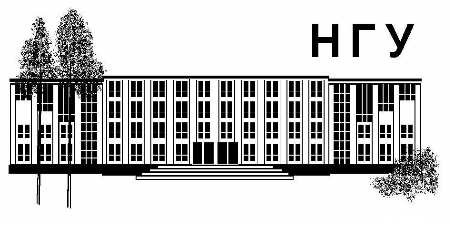
\includegraphics[width=0.23\textwidth]{../NSU-logo}

    Кафедра теоретической физики физического факультета НГУ
    \medskip

    \Large
    Профессор Фадин В.\,С.
    \bigskip

    \huge
    \textbf{Квантовая электродинамика}
    \bigskip

    \Large
    Лекция № 8
    \vfill

    \normalsize
    % \begin{minipage}{0.65\linewidth}
    % \end{minipage}
    \vfill

    \normalsize \ccbysa\hspace{0.5em}  Новосибирск 2013
  \end{center}
\end{titlepage}
\vspace*{-1em}
\begin{center}
\vfill
  \begin{minipage}{0.75\linewidth}
    Гамильтониан Брейта. Уровни энергии позитрония. Ортопозитроний и
    парапозитроний. Cвязь ширины распада орто- и паразитрония с
    сечением аннигиляции электрон"=позитронной пары в два и три фотона
    на пороге. Комптон"=эффект. Аналогия с сечением рассеяние фотона на
    точечной заряженной скалярной частице: диаграммы Фейнмана,
    матричный элемент (построение диаграммной техники для скалярной
    электродинамики из требования калибровочной инвариантности),
    удобство системы покоя начальной частицы и выбора физических
    поляризаций фотонов, суммирование по физическим поляризациям
    фотонов.  Переход к сечению рассеяния фотона на
    электроне. Сравнение поведения сечений рассеяния фотона на частице
    со спином 0 и $1/2$ в нерелятивизме и ультрарелятивизме. Разложение
    амплитуды по парциальным волнам и кросс-инвариантность:
    энергетическая зависимость амплитуд и сечений при больших энергиях
    и фиксированных передачах импульсов (реджевская асимптотика).
  \end{minipage}
  \vfill

  \normalsize \ccbysa\hspace{0.5em} Новосибирск 2013
\end{center}
\end{document}
